\section{Empirical Findings}

\begin{figure}[t]
    \centering
    \begin{minipage}{0.32\textwidth}
        \centering
        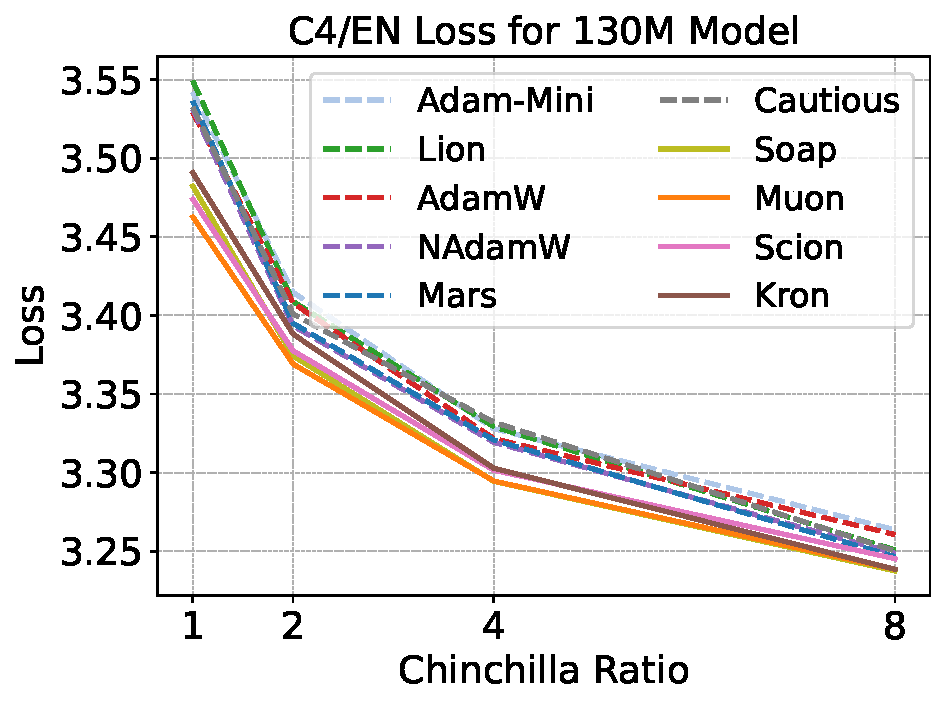
\includegraphics[width=\linewidth]{figures/optimizer_loss_scaling_130m.pdf}
    \end{minipage}%
    \hfill
    \begin{minipage}{0.32\textwidth}
        \centering
        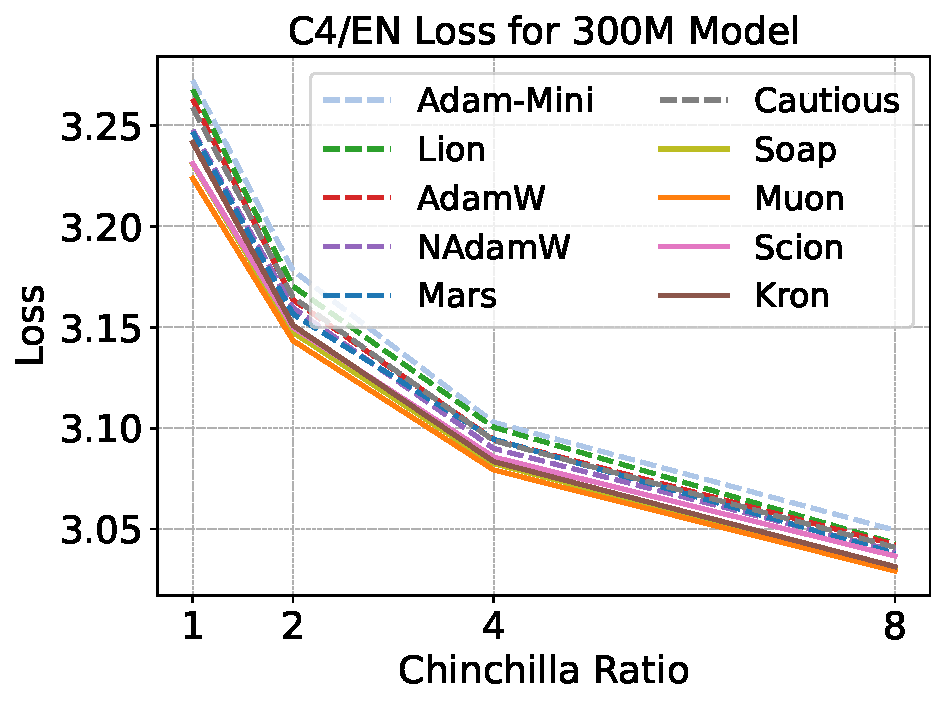
\includegraphics[width=\linewidth]{figures/optimizer_loss_scaling_300m.pdf}
    \end{minipage}%
    \hfill 
    \begin{minipage}{0.32\textwidth}
        \centering
        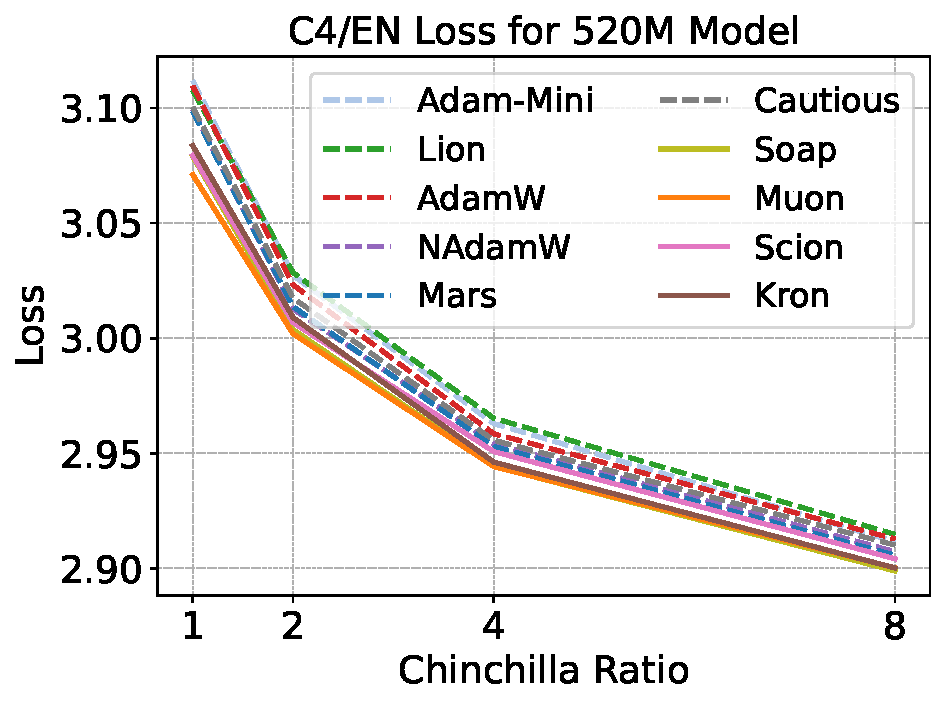
\includegraphics[width=\linewidth]{figures/optimizer_loss_scaling_520m.pdf}
    \end{minipage}%

    \begin{minipage}{0.32\textwidth}
        \centering
        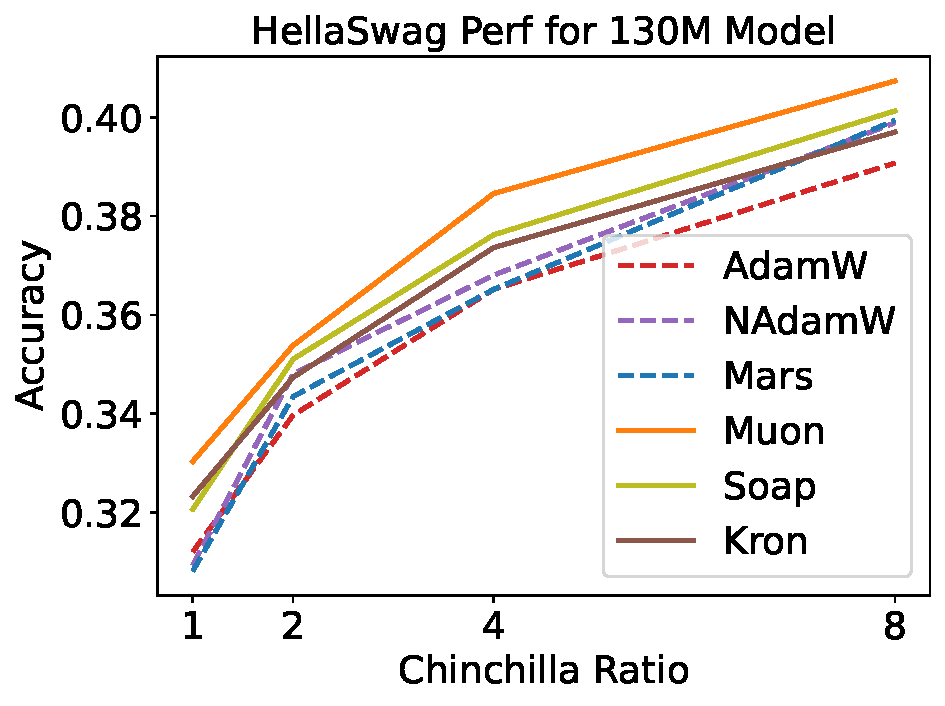
\includegraphics[width=\linewidth]{figures/hellaswag_0shot_130m.pdf}
    \end{minipage}
    \begin{minipage}{0.32\textwidth}
        \centering
        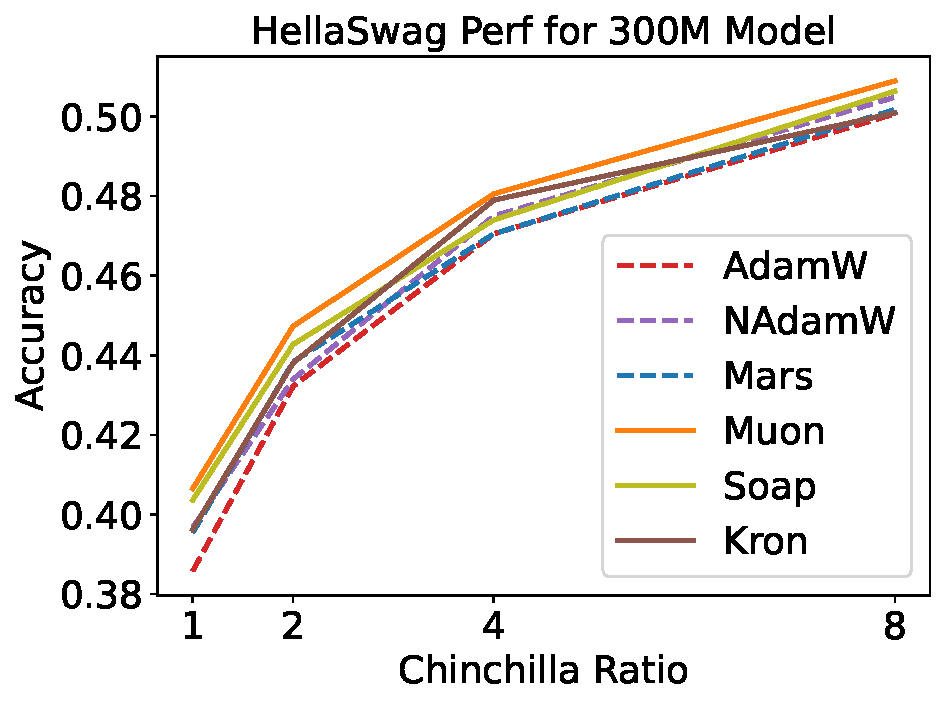
\includegraphics[width=\linewidth]{figures/hellaswag_0shot_300m.pdf}
    \end{minipage}
    \begin{minipage}{0.32\textwidth}
        \centering
        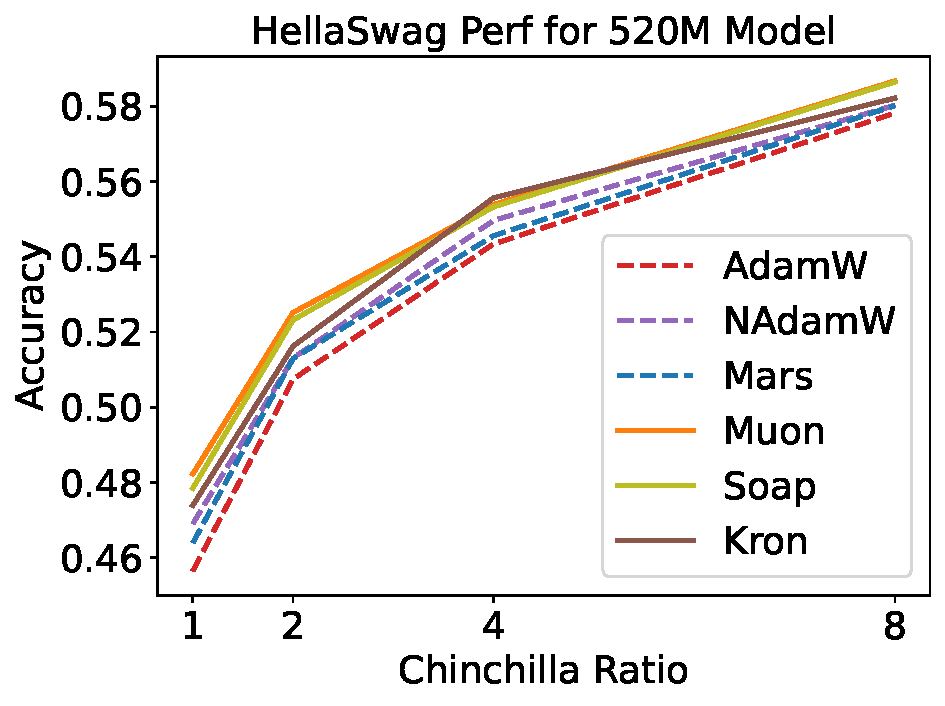
\includegraphics[width=\linewidth]{figures/hellaswag_0shot_520m.pdf}
    \end{minipage}
    \caption{\textbf{Main Results For Phase I \& II.} Top: We plot the validation loss on C4/EN for the experiments in Phase I and Phase II. Every point corresponds to the optimal loss achieved at the corresponding Chinchilla ratio for each optimizer. Bottom: we plot the HellaSwag performance corresponding to the selected run for a subset of optimizers: the AdamW baseline, the top 2 most performant scalar-based optimizers, and the top 3 most performant matrix-based optimizers. Analysis is deferred to~\Cref{sec:opt-comp-gen}.}
    \label{fig:main}
\end{figure}





\begin{figure}[t]
    \begin{minipage}{0.32\textwidth}
        \centering
        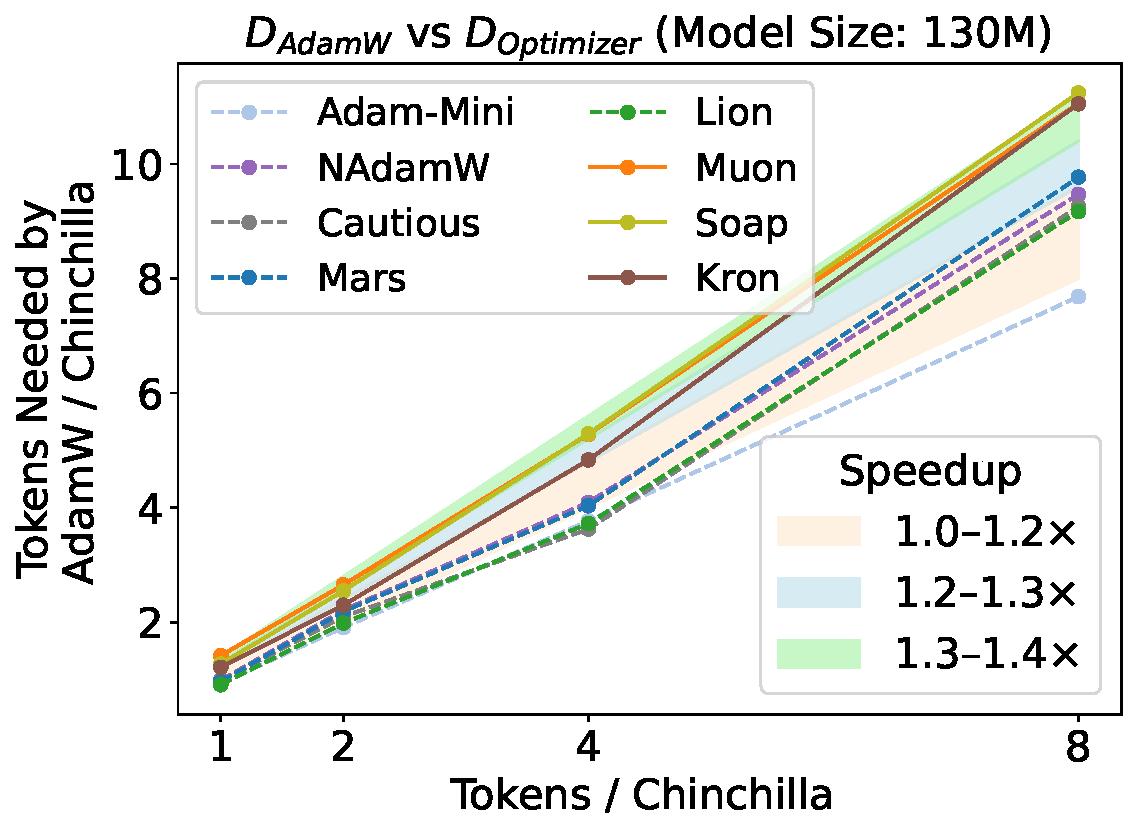
\includegraphics[width=\linewidth]{figures/D_eff_vs_D_opt_130mM.pdf}
    \end{minipage}
    \hfill
    \begin{minipage}{0.32\textwidth}
        \centering
        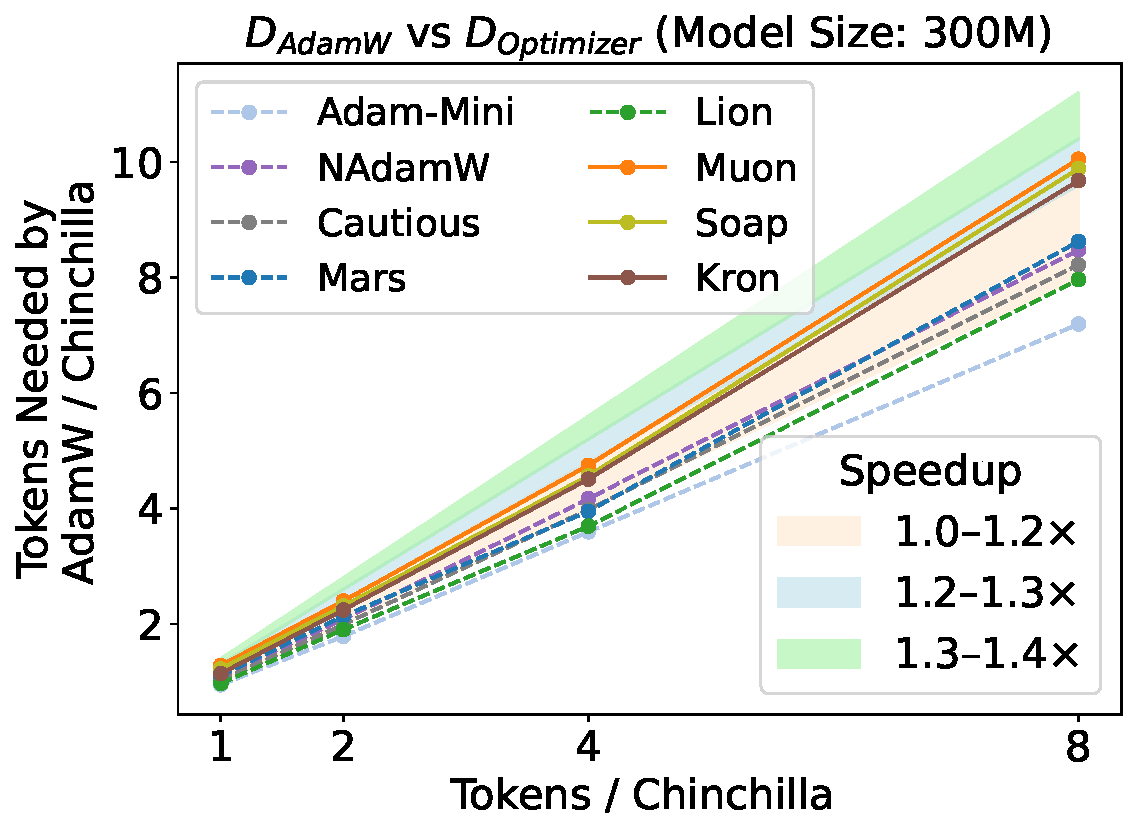
\includegraphics[width=\linewidth]{figures/D_eff_vs_D_opt_300mM.pdf}
    \end{minipage}
    \hfill
    \begin{minipage}{0.32\textwidth}
        \centering
        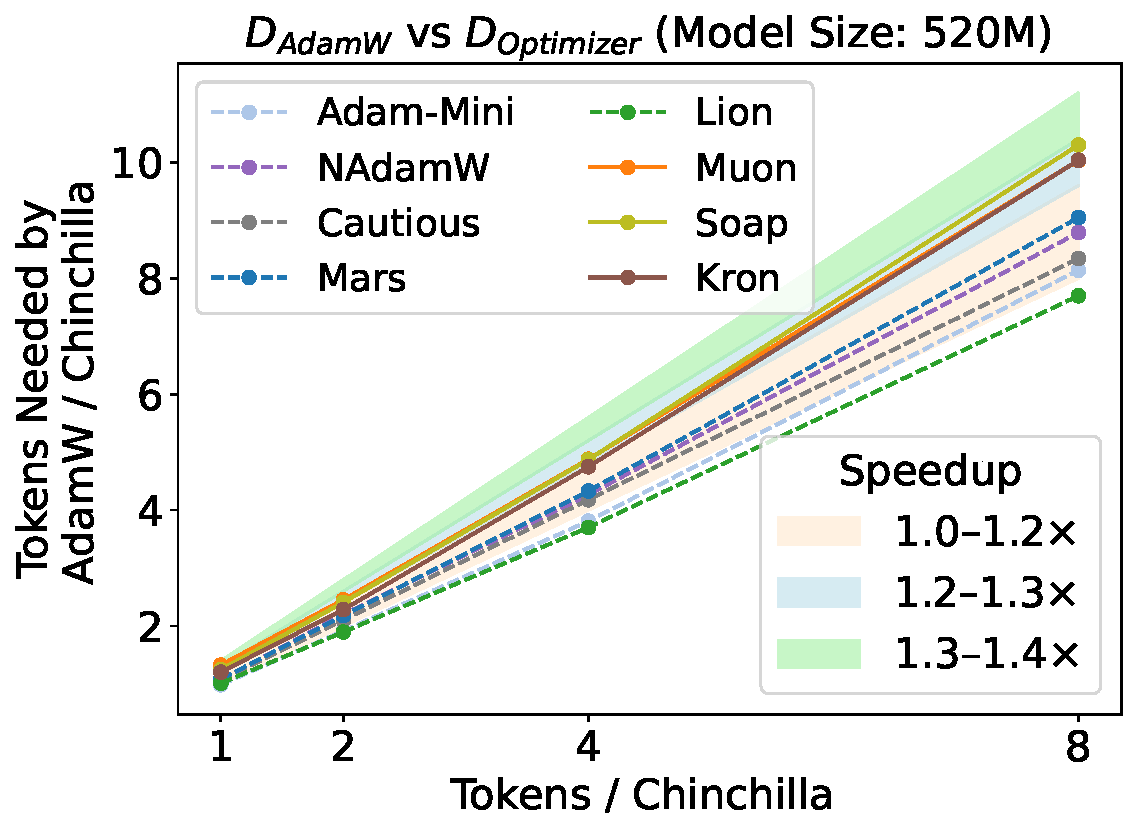
\includegraphics[width=\linewidth]{figures/D_eff_vs_D_opt_520mM.pdf}
    \end{minipage}
    \caption{\textbf{Speedup of different optimizers across scale.} We estimate the speedup of different optimizers by fitting a scaling law for AdamW and then map the loss of different optimizers to the corresponding equivalent data budget. We observe that (i) The highest speedup is capped at 1.4$\times$; (ii) matrix-based optimizers consistently outperform scalar-based optimizers and show an increasing speedup with data budget.}
    \label{fig:speedup}
\end{figure}



\subsection{Main Results}
\label{sec:opt-comp-gen}

\paragraph{Results on 0.1B–0.5B-parameter models.} 
Figure~\ref{fig:main} shows the validation loss curves for the 130M, 300M, and 520M models with varying Chinchilla ratios (1 to 8) in our benchmark. We further show that HellaSwag accuracy improvements closely mirror validation-loss gains. This is consistent with prior works that show lower losses translates to better downstream accuracy~\cite{bhagia2024establishingtaskscalinglaws,liu2025regmixdatamixtureregression}.
Across all model scales and compute budgets, both the variance-reduced Adam variants (NAdamW, Mars, Cautious) and the matrix-based optimizers deliver speedups over the AdamW baseline.  However, no method achieves $2\times$ step-wise acceleration claimed in previous literature. We note that Soap~\cite{vyas2025soapimprovingstabilizingshampoo} is one of the few works that conduct independent hyperparameter sweeping for the baseline, and it indeed reports a speedup closest to the actual observed improvement.
Following the methodology defined in~\Cref{sec:phase2}, we calculate the estimated speedup ratio of different optimizers in~\Cref{fig:speedup} and the highest speedup ratio is 1.4$\times$. 
From the measured speedups, three  patterns stand out in this computation regime:

\begin{enumerate}[leftmargin=*]
\item \textit{Matrix-based methods outperform scalar-based methods. The speedup ratio increases with data budget yet decreases with model size.}
For every model size, matrix-based optimizers (Soap, Muon, Kron, Scion—solid curves) consistently drive validation loss below that of their scalar-based counterparts (dashed curves). In the base (1$\times$ Chinchilla) compute regime, Muon performs best, but at 8× Chinchilla compute, the advantage shifts to Soap and Kron. As shown by the super-linear trend in Figure~\ref{fig:speedup}, the speedup ratios of these three optimizers grow with increasing data budget. To the best of authors' knowledge, this dependency on data budget is not noted in prior works, which typically only experiment on one data-to-model ratio.

However, the greatest gains occur on the 130M model, after which the speedup decreases to roughly 1.3× for larger model sizes. We will affirm this observation further in the experiments of 1.2B models, showing that the speedup ratios of matrix-based optimizers decrease to 1.1$\times$ for the 1.2B model.

\item \textit{Variance-reduction techniques provide a small but clear lift.}
Within the scalar-based family, all variance-reduced Adam variants ({NAdamW}, {Mars}, {Cautious}) consistently surpass vanilla AdamW---except for a small lag at the smallest experiment. Notably, {Muon} combines matrix-based updates with Nesterov momentum, illustrating how variance reduction compounds with matrix adaptation can yield greater efficiency. This result is vastly different from the $2\times$ speedup reported in some of the works and we attribute this disparity to the better-tuned baseline.


\item \textit{Memory-efficient variants of AdamW closely track the performance of AdamW.} 
The two memory-efficient AdamW variants ({Lion}, {Adam-mini})—despite their reduced auxiliary state—closely track the performance of AdamW, with a slowdown of at most $5\%$ and sometimes even perform better than AdamW. Interestingly, Lion and Adam-mini show different scaling trends regarding model size: the disadvantage of Lion relative to AdamW widens while the disadvantage of Adam-mini over AdamW narrows. 
\end{enumerate}











\begin{figure}
    \begin{minipage}{0.32\textwidth}
        \centering
        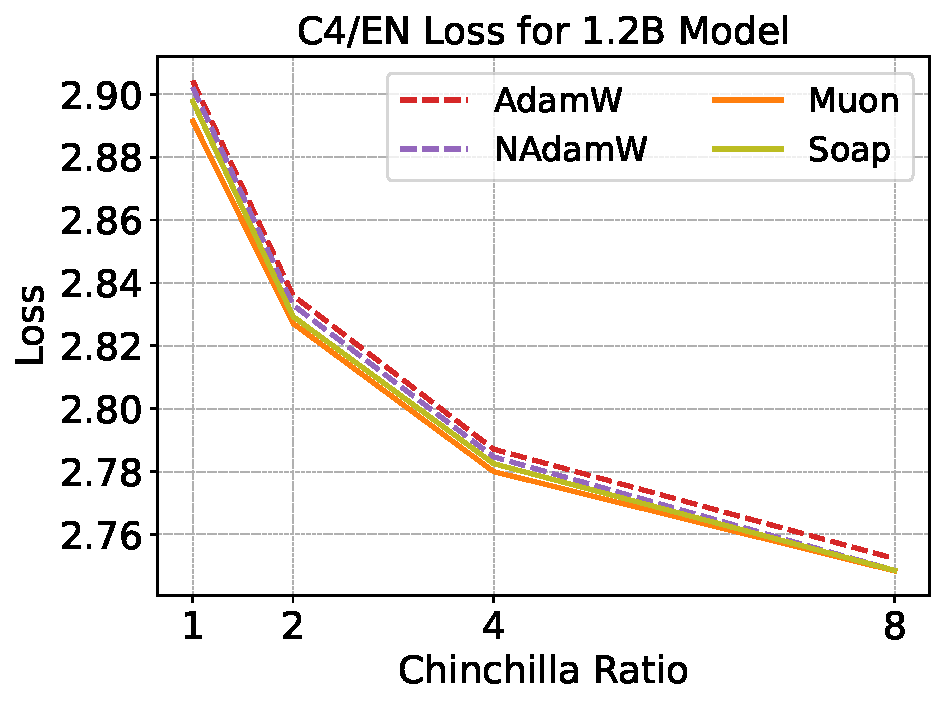
\includegraphics[width=\linewidth]{figures/optimizer_loss_scaling_1.2b.pdf}
    \end{minipage}
    \hfill
    \begin{minipage}{0.32\textwidth}
        \centering
        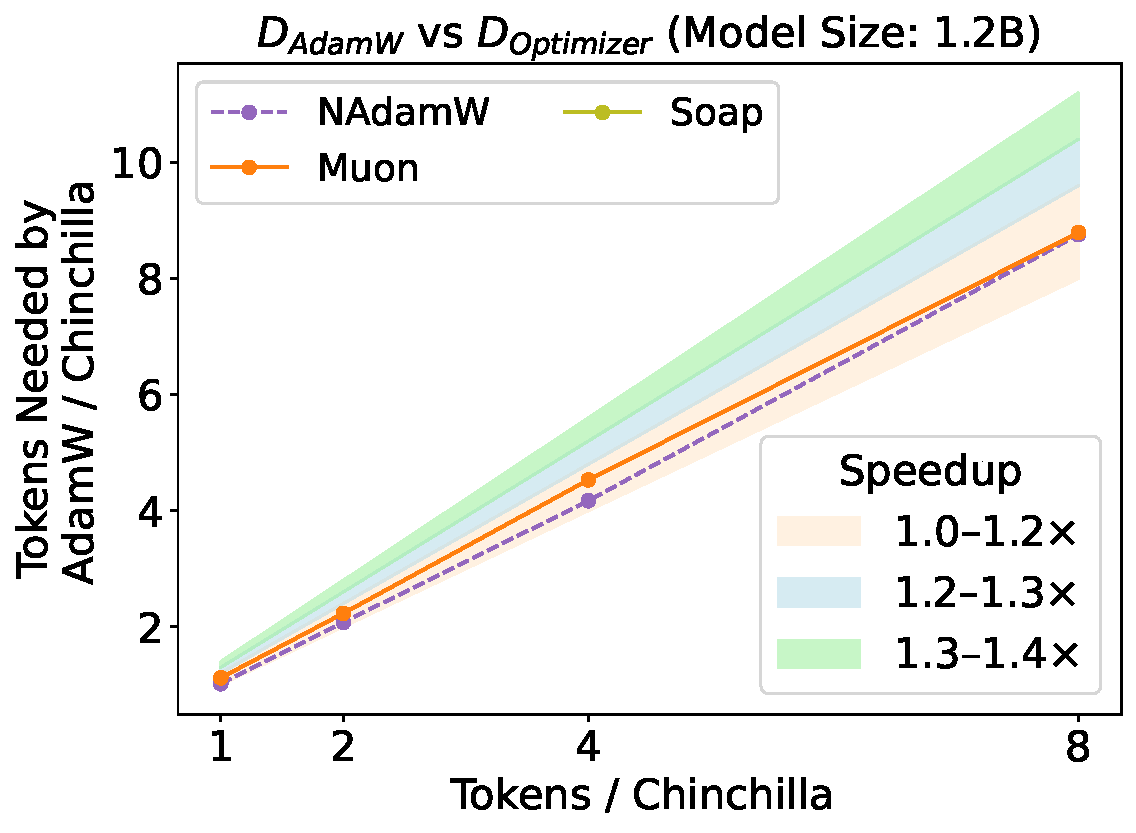
\includegraphics[width=\linewidth]{figures/D_eff_vs_D_opt_1.2bM.pdf}
    \end{minipage}
    \hfill
    \begin{minipage}{0.32\textwidth}
        \centering
        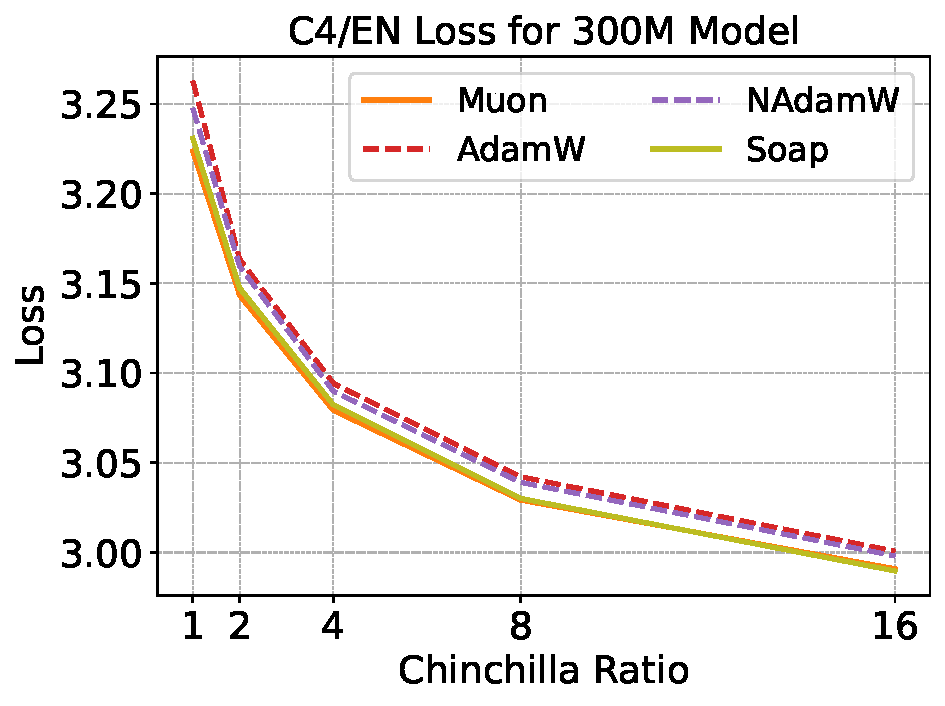
\includegraphics[width=\linewidth]{figures/final2.pdf}
    \end{minipage}
    \caption{\textbf{Case Studies.} Left: Validation loss scaling on 1.2B model for AdamW, NAdamW, Muon and Soap. Muon and Soap still offer significant speedup over AdamW but no longer significantly speed up over NAdamW. Mid: Estimated speedup ratio with the same methodology~\Cref{fig:speedup}, we observe that Muon and Soap's speedup decays with model size to only $1.1\times$. Last: Experiment with 300M $16 \times$ Chinchilla setting, Soap outperforms Muon when data-to-model ratio further increases.}
    \label{fig:case}
\end{figure}

\paragraph{Results on 1.2B-parameters Models.}
Using the hyperparameter scaling law we fit (\Cref{sec:phase2}), we scale up the model size to 1.2B to examine how the speedup of optimizers scales with model size. We observe that NAdamW, Muon, and Soap still deliver speedup over AdamW, but the speedup deminishes to $\approx$1.1$\times$ for all these optimizers (\Cref{fig:case}, Left and Mid) and no longer leads to downstream improvements (\Cref{tab:benchmark}). Based on this observation, we fit scaling laws for both AdamW and Muon based on the loss of 16 runs, and our scaling law predicts that Muon will result in a slightly higher loss than AdamW in the $7$B and $1\times$ Chinchilla regime. We defer the fitting procedure to~\Cref{app:scaling_law}.


\setlength{\tabcolsep}{3pt}
\begin{table}[h]
  \centering
  \caption{Benchmark performance of 1.2B models with different optimizers and Chinchilla scaling.}
  \label{tab:bench-1p2b}
  \small
  \begin{tabular}{ll*{10}{c}}
    \toprule
    Optimizer 
      & LAMBADA & OpenBook & Wino & PIQA & BoolQ 
      & WSC273 & Hella & ARC-C. & ARC-E & COPA & Avg \\
    \midrule
      \multicolumn{12}{c}{\textbf{8x Chinchilla (193B)}} \\
     AdamW  & 67.16 & 41.40 & 64.96 & 76.12 & 68.59 
      & 82.78 & 67.56 & 43.43 & 74.49 & 85.00 & 67.15 \\
     NAdamW & 67.84 & 40.20 & 64.80 & 77.15 & 68.10 
      & 83.52 & 67.40 & 43.34 & 73.61 & 81.00 & 66.70 \\
    Muon  & 67.53 & 39.80 & 67.09 & 77.09 & 68.81 
            & 80.95 & 67.67 & 43.34 & 73.53 & 84.00 & {66.98} \\
    \bottomrule
  \end{tabular}
  \label{tab:benchmark}
\end{table}

\textbf{High data-to-model Ratio.} In our previous experiments, Muon is outperformed by Soap in the 8$\times$ Chinchilla regime for the 130M and 520M models. To further test this, we train three 300M models to 16$\times$ Chinchilla and verify that Muon is no longer the optimal optimizer when the data-to-model ratio increases (\Cref{fig:case}, right). We conjecture that the second-order momentum maintained by Soap and Kron becomes more effective when the data-to-model ratio increases. In the long run, adaptivity to heterogeneity in parameter directions may lead to a larger speedup. We also perform similar experiments on 130M models and reach the same results (deferred to~\Cref{app:more_overtrained}).









\subsection{Necessity of Rigorous Benchmarking}

Our systematic sweeps uncover both universal optimization principles and surprising optimization-specific nuances, which call for rigorous study when designing future optimizers. 



First, we find that even a superior optimizer can underperform a less advanced method when its hyperparameters are not precisely tuned. In our exhaustive grid searches, slight deviations from each optimizer's ideal learning rate or other critical hyperparameter often lead to degradation in validation loss that is large enough to flip the ordering (\Cref{fig:necessity}, Left). This hyperparameter sensitivity means manual selection without systematic sweeps will likely produce arbitrary ranking of the optimizers. To further demonstrate this, we plot how validation losses vary  when only \textbf{one} of the hyperparameters deviates from optimal value for {Muon}, {Soap}, {Mars} on 520M model in 1$\times$ Chinchilla regime (\Cref{fig:necessity}, Mid). The ordering of the optimizers can easily flip if one chooses a sub-optimal hyperparameter.




Second, using the same hyperparameters for different optimizers do not guarantee fair comparison between optimizers. For example, while weight decay is essential across all optimizers for optimal performance, the optimal decay strength varies markedly between optimizers. As shown in (\Cref{fig:motivation}, top right), optimal weight decay coefficients differ between the optimizers studied. We also note the optimal weight decay for Kron is larger than the conventional $0.1$ and is approximately $0.5$, which is crucial for Kron to outperform AdamW. 

Third, early training behavior can be highly misleading. Validation-loss curves during this initial phase tend to exaggerate performance gaps (\Cref{fig:motivation}, bottom right) and, in some cases, even reverse the eventual ranking, (\Cref{fig:necessity}, right). Many optimizers exhibit rapid early descent followed by plateauing, meaning that assessments based solely on losses before the end of the training  trajectories fail to predict final outcomes. To avoid such pitfalls, we recommend evaluating optimizers only on the final checkpoints rather than relying on intermediate checkpoints (e.g. in~\cite{liu2025muonscalablellmtraining}). 

We also note that the evaluaton in Sophia~\cite{liu2024sophiascalablestochasticsecondorder} largely follows the correct procedure of the comparisons above --- the peak learning rate was tuned to be optimal for the baseline. However, as the data loader in the codebase used did not fully randomize the order of the data, the optimal peak learning rate in that code base for AdamW is significantly smaller than the optimal peak learning rate for a fully randomized data loader setting. It turns out that Sophia doesn't offer significant speedup over AdamW for models under 0.5B in our setting (\Cref{fig:sophia_experiments}).

\begin{figure}[t]
    \begin{minipage}{0.48\textwidth}
        \centering
        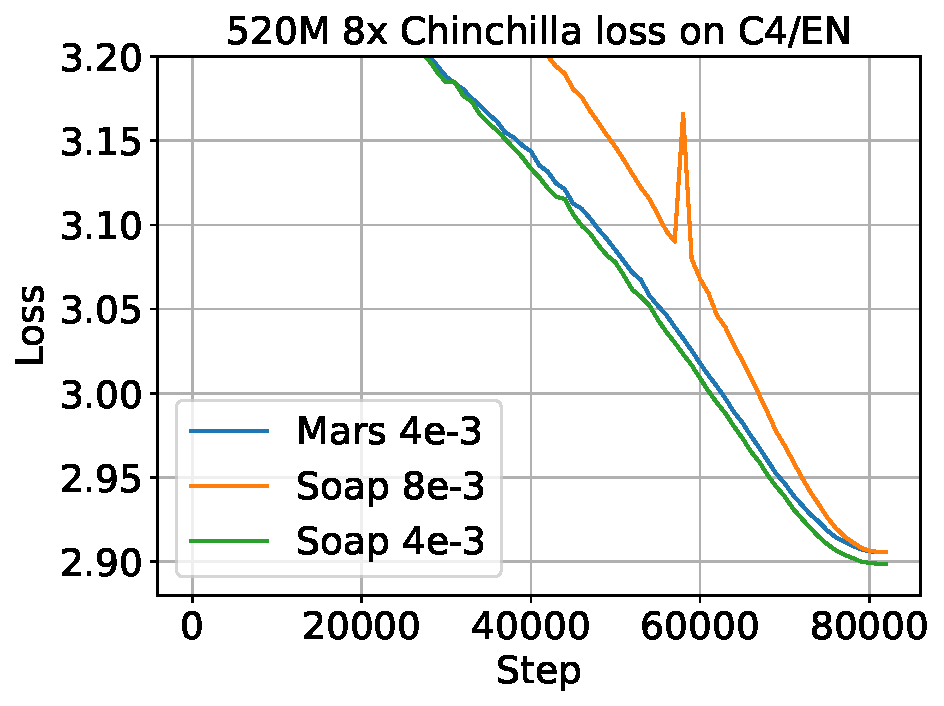
\includegraphics[width=\linewidth]{figures/lr_matters.pdf}
    \end{minipage}
    \hfill
        \begin{minipage}{0.48\textwidth}
        \centering
        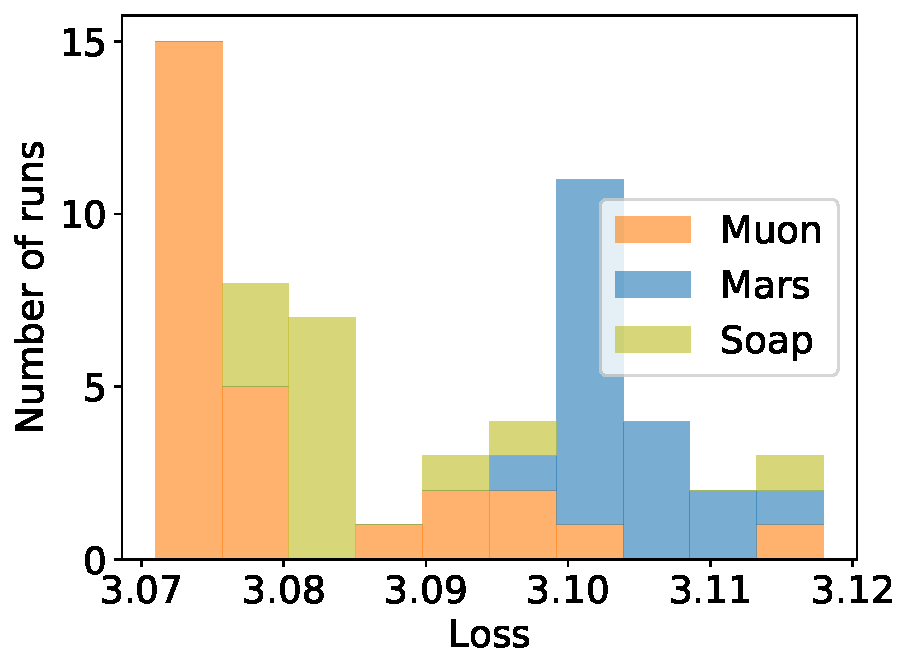
\includegraphics[width=\linewidth]{figures/loss_hist.pdf}
    \end{minipage}
    \hfill
    \begin{minipage}{0.48\textwidth}
        \centering
        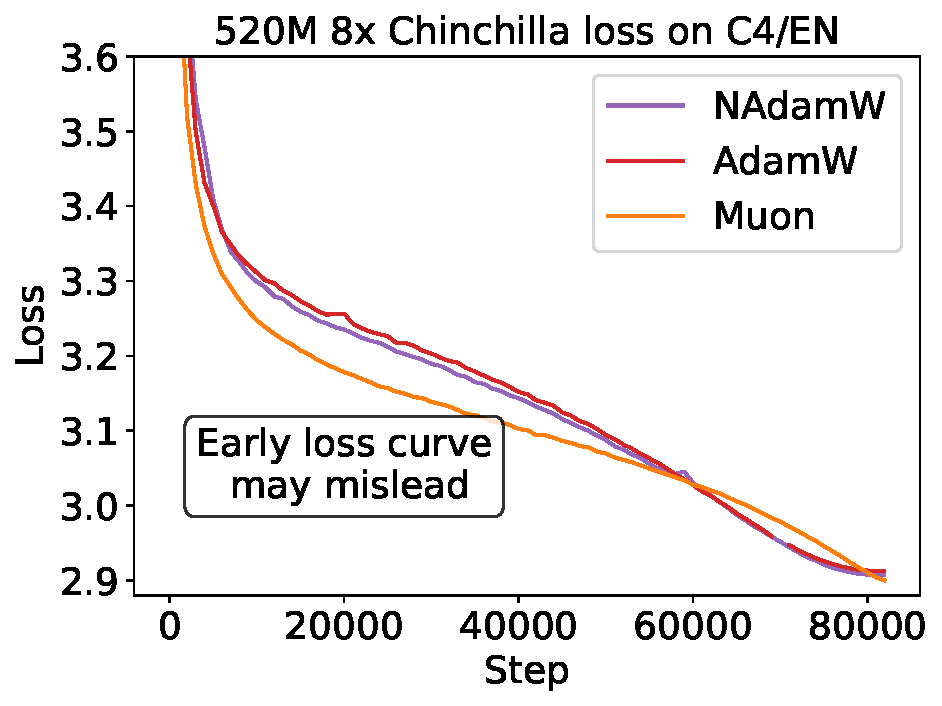
\includegraphics[width=\linewidth]{figures/multiple_crossing.pdf}
    \end{minipage}%
    \hfill
    \begin{minipage}{0.48\textwidth}
        \centering
        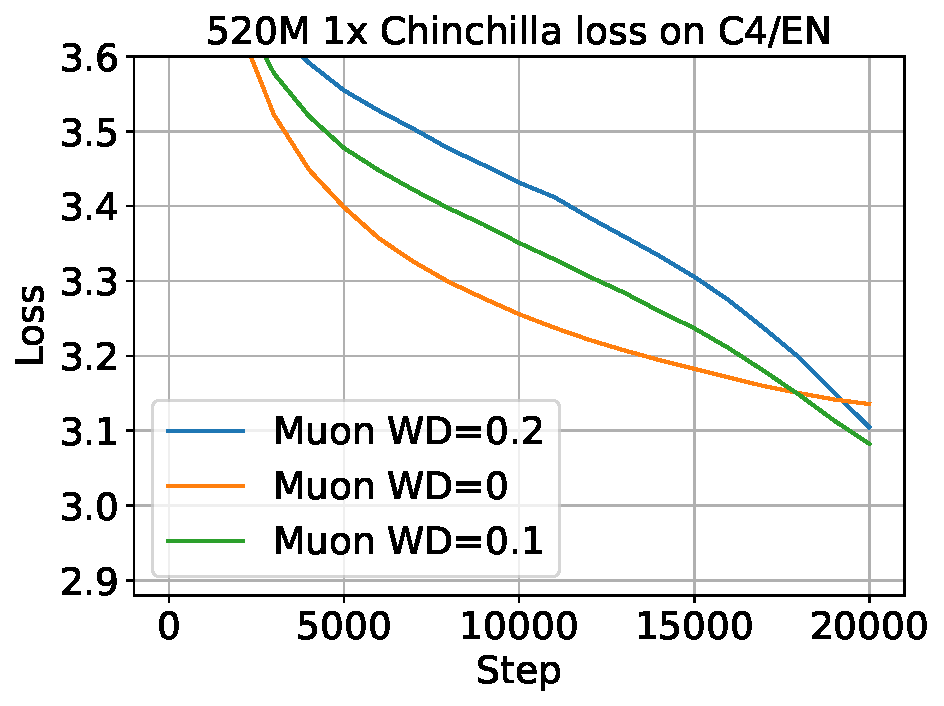
\includegraphics[width=\linewidth]{figures/multiple_crossing_same_optimizer.pdf}
    \end{minipage}
    
    \caption{\textbf{Necessity of Careful Tuning.} Left: 2$\times$ the optimal learning rate diminishes Soap's loss improvement over Mars on 520M 8x experiment; Mid: Variation of loss when only one hyperparameter differs from optimal learning rate and runs converge to within $0.02$ of optimal. The order of optimizers may flip arbitrarily if rigorous tuning is missing. Right: Changing a single hyperparameter like weight decay may lead to misleading faster loss improvement but plateaus later.}
    \label{fig:necessity}
\end{figure}



\begin{figure}
    \begin{minipage}{0.24\textwidth}
        \centering
        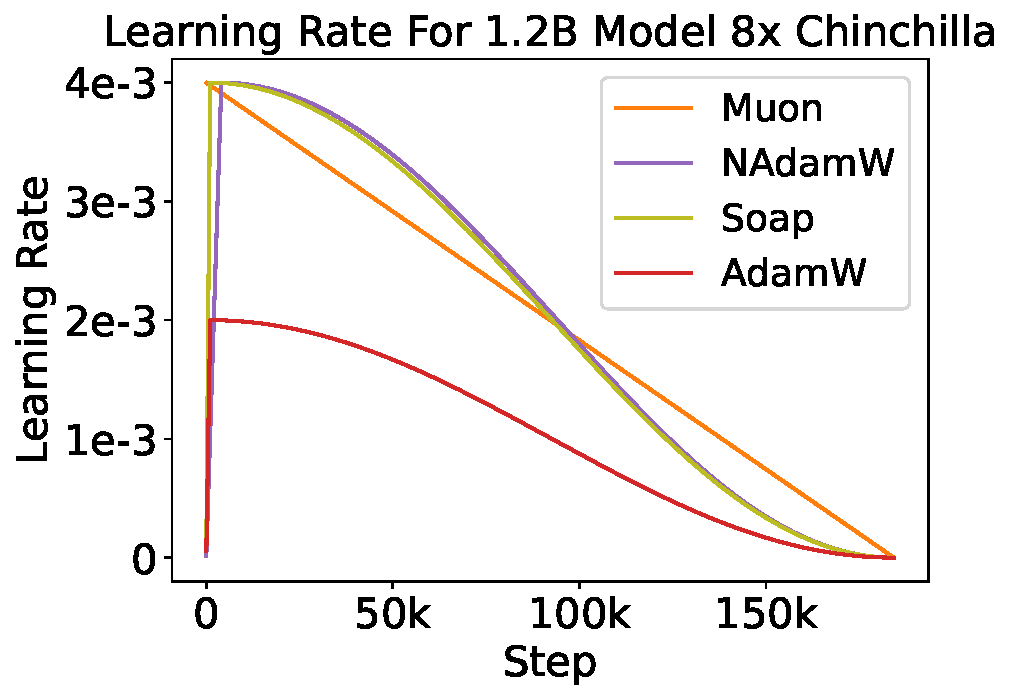
\includegraphics[width=\linewidth]{figures/lr.pdf}
    \end{minipage}
    \hfill
    \begin{minipage}{0.24\textwidth}
        \centering
        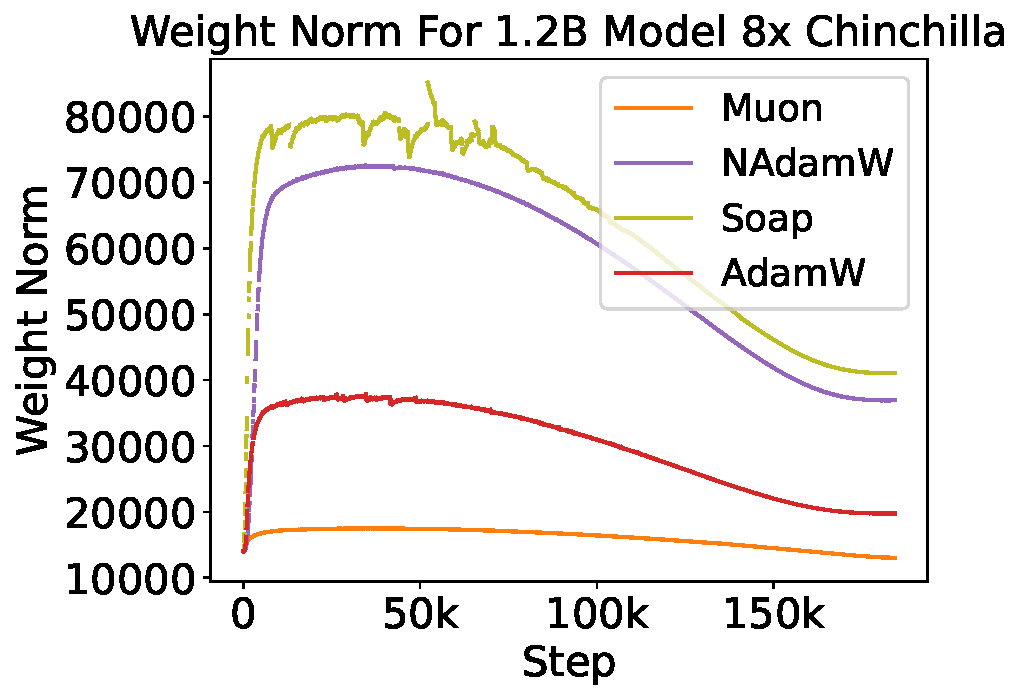
\includegraphics[width=\linewidth]{figures/norm.pdf}
    \end{minipage}
    \hfill
    \begin{minipage}{0.24\textwidth}
        \centering
        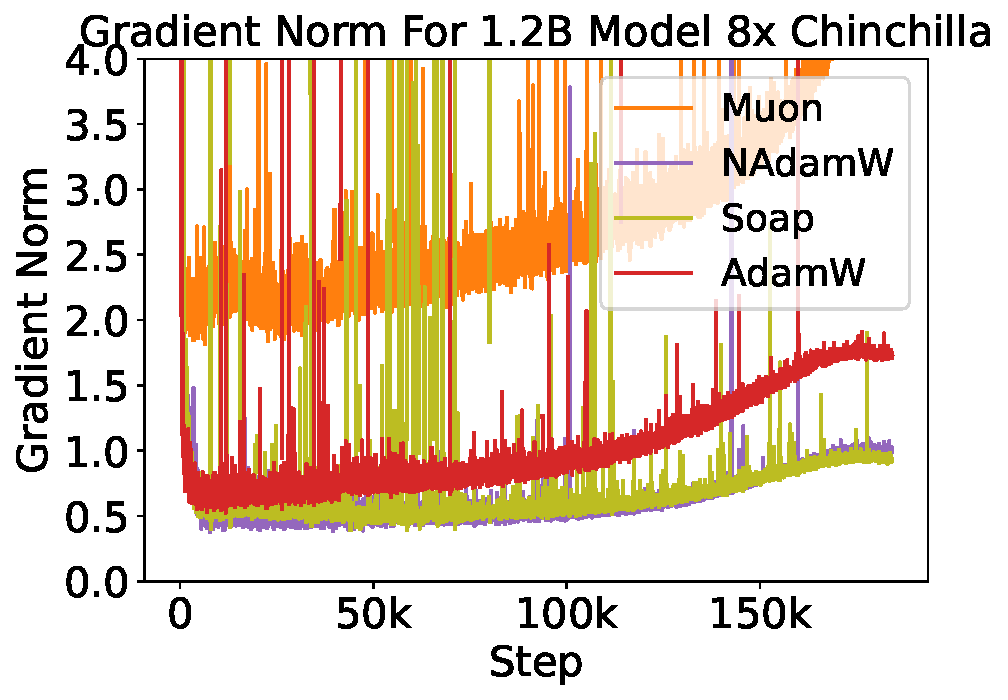
\includegraphics[width=\linewidth]{figures/normg.pdf}
    \end{minipage}
    \hfill
    \begin{minipage}{0.24\textwidth}
        \centering
        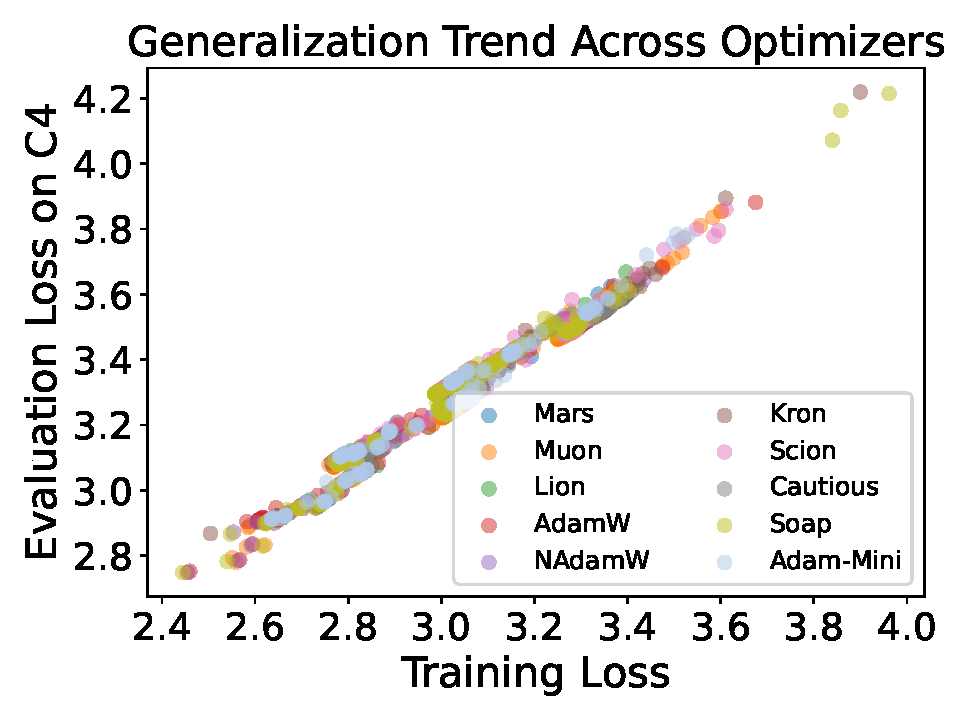
\includegraphics[width=\linewidth]{figures/two_losses.pdf}
    \end{minipage}
    \caption{\textbf{Common  Phenomena Across Optimizers.} 
    \textbf{Left}: Learning rate used for different optimizers.
    \textbf{Middle Left}: Parameter norm of all optimizers shows a similar trend of increment and decrease, closely aligning the increasing and decaying of learning rate schedule. \textbf{Middle Right}: Gradient norm increases during learning rate decay. However, this increase does not lead to a loss increase. \textbf{Right}: The training loss and evaluation loss follows the same trend for all optimizers.}
    \label{fig:common}
\end{figure}


\subsection{Common Phenomena Across Optimizers}


Through logging the evolution of weight and gradient norms, we discovered some shared optimization phenomena across optimizers.

\textbf{Parameter norms typically track learning rate decay when there is weight decay} We observe that the parameter norms of all optimizers show a similar pattern of increase and decrease, closely aligning with the increase and decrease of the learning rate if there is a decay phase. However, the absolute values of parameter norms are very different across optimizers (Figure~\ref{fig:common}, Middle Left).

\textbf{Gradient norm increases during learning rate decay.} Across all the optimizers, the gradient norms increase during the training run. However, this increase does not lead to a loss increase. Similar to the parameter norms, the absolute values of gradient norms are not consistent across optimizers.
These two phenomena are also reported in the previous work~\cite{defazio2025gradientsrapidlyincreasenear}, where the author also provides a theoretical explanation for both phenomena. We provide additional evidence that these two phenomena are not artifacts of the chosen optimizer AdamW but rather common phenomena across optimizers (Figure~\ref{fig:common}, Middle Right).


\textbf{Different optimizers have similar generalization behavior.} For architecture design, it has been observed that different architectures can have vastly different generalization behaviors~\cite{lu2025doessequencemodelingarchitecture}. However, this is not the case for optimizers, and the evaluation losses and training losses follow roughly the same trend for all optimizers at the regimes we experimented on (Figure~\ref{fig:common}, Right).







